\documentclass{article}
\usepackage{arxiv}

\usepackage[utf8]{inputenc}
\usepackage[english]{babel}
\usepackage[T1]{fontenc}
\usepackage{url}
\usepackage{booktabs}
\usepackage{amsfonts}
\usepackage{nicefrac}
\usepackage{microtype}
\usepackage{lipsum}
\usepackage{graphicx}
\usepackage{float}
\usepackage{wrapfig}
\graphicspath{{../figures}}
\usepackage[square,numbers]{natbib}
\bibliographystyle{abbrvnat}
\usepackage{amsmath}
\usepackage{caption}
\usepackage{subcaption}
\usepackage{doi}
\usepackage{algorithm}
\usepackage{algpseudocode}
\usepackage{amssymb}

\usepackage{doi}


\title{Differential neural ensemble search with diversity control}

\author{P. Babkin, K. Yakovlev, K. Petrushina, O.Bakhteev,
	%% David S.~Hippocampus\thanks{Use footnote for providing further
	%%	information about author (webpage, alternative
	%%	address)---\emph{not} for acknowledging funding agencies.} \\
	%%Department of Computer Science\\
	%%Cranberry-Lemon University\\
	%%Pittsburgh, PA 15213 \\
	%%\texttt{hippo@cs.cranberry-lemon.edu} \\
	%% examples of more authors
	%%\And
	%%Elias D.~Striatum \\
	%%Department of Electrical Engineering\\
	%%Mount-Sheikh University\\
	%%Santa Narimana, Levand \\
	%%\texttt{stariate@ee.mount-sheikh.edu} \\
	%% \AND
	%% Coauthor \\
	%% Affiliation \\
	%% Address \\
	%% \texttt{email} \\
	%% \And
	%% Coauthor \\
	%% Affiliation \\
	%% Address \\
	%% \texttt{email} \\
	%% \And
	%% Coauthor \\
	%% Affiliation \\
	%% Address \\
	%% \texttt{email} \\
}
\date{}

\renewcommand{\shorttitle}{differentiable ensembles search}

%%% Add PDF metadata to help others organize their library
%%% Once the PDF is generated, you can check the metadata with
%%% $ pdfinfo template.pdf
\hypersetup{
pdftitle={Differentiable algorithm for searching ensembles of deep learning models with diversity control},
pdfsubject={q-bio.NC, q-bio.QM},
pdfauthor={P.Babkin, K.Petrushina, K.Yakovlev, O.Bakhteev},
pdfkeywords={First keyword, Second keyword, More},
}

\begin{document}
\maketitle

\begin{abstract}
	
In our research, we investigate a novel method for sampling deep learning models using a hypernetwork. The hypernetwork is a neural network that controls the diversity of the models by translating a real number representing ensemble diversity into a sampled neural network architecture. Architectures are obtained in a one-shot manner by perturbing from the base architecture in terms of the Jenson-Shannon divergence (JSd). We evaluate the performance of the proposed algorithm by conducting experiments on the Fashion-MNIST and CIFAR-10 datasets, comparing the resulting ensembles with those sampled by other searching algorithms.

\end{abstract}


\keywords{ differential search \and neural ensembles \and hypernetwork \and diversity control }

\section{Introduction}

Nowadays methods of neural architecture search (NAS) are well-explored and proved to be an effective way of creating
more effective and efficient neural networks \citep{darts, robustify, xnas}. Some of these methods use different ways to smooth out the architecture so optimum for it can
be found by wide range of methods for smooth optimization problems. On the other hand, neural ensemble search (NES) is
modern and not as well investigated problem as NAS, although it is known that ensembles of deep learning models show better
results in different applied problems \citep{multi-head}.
Our paper investigates the method of sampling deep learning models in a new way that gives compatible results and has its own sphere
of implementations.

Our method takes the result of NAS as a base architecture than it samples architectures which are close to the optimal one in terms of Jensen-Shannon divergence (JSd).
JSd is used to measure distance between two distributions and is symmetric and finite in contrast to more popular Kullback–Leibler divergence. In our investigation we consider preferences of operations between nodes of architecture to be a discrete distribution so we can measure distance between them in terms of JSd.

Architectures differ in terms of $\lambda$, idea of method is shown in \hyperref[fig:arch]{Fig. 1}. Basic architecture is gained with $\lambda = \lambda_1$.
Blue ellipses are equidistant surfaces of architectures. Staring with diverse parameter $\lambda = \lambda_2$ resulting architecture performs unacceptable accuracy, so architectures beyond the surface are not included into ensemble.
Method can control whether sampled architectures are close enough to the optimal one so they perform good accuracy on the original dataset and are diverse enough so every architecture makes its own contribution to the final answer.

\begin{figure}[h]
    \centering
    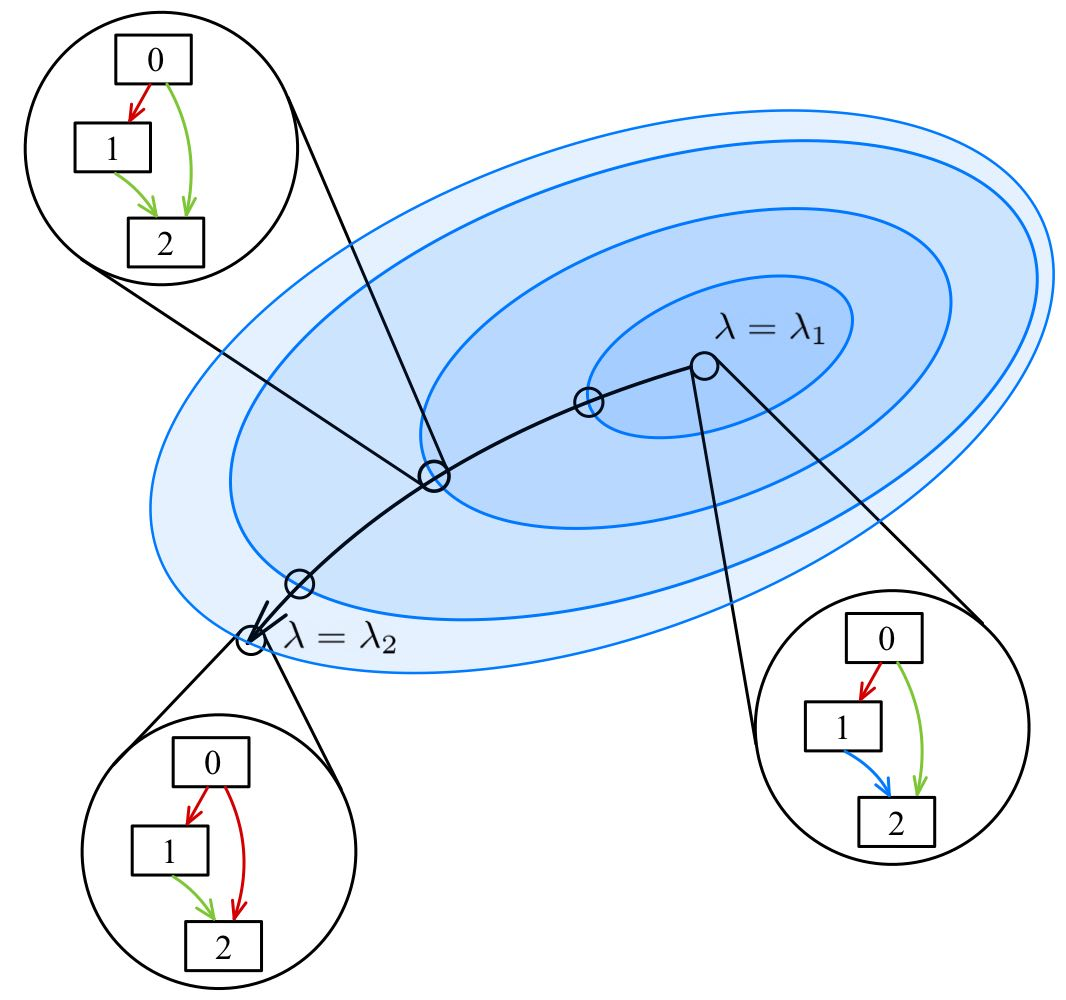
\includegraphics[width=0.6\textwidth]{fig1}
    \caption{\label{fig:arch}Architecture space with JSd metrics.
    Blue ellipses are equidistant surfaces. The space is continuous but has varying preferred operations across different architectural levels. Architectures with different operations are pictured separately on the picture.}
\end{figure}

To sample architectures we use hypernetwork \citep{hypernetworks}. This network generates parameters for another network, which is called target network.
Previously hypernetwoks were intended to control different characteristics such as
complexity of architecture \citep{darts-cc} or parameters of the target model \citep{cont-learn} in several modern papers. In our paper it controls 
diversity of the target models, so every sampled model differs from previously sampled ones in terms of JSd.

The hypernetwork uses JSd to measure difference between two architectures. Our main idea of sampling different model is to use a regularizer,
based on JSd as a source of diversity.

This way we sample deep learning models in one-shot unlike NES
for Uncertainty Estimation \citep{nes}, where every sampled models must be tested and least appropriate architectures are excluded from ensemble.
In this way our method is similar to NES via Bayesian Sampling \citep{baysiannes}, but we sample architectures using different approach, posterior distribution for architectures is gained based on the optimal one.
To sum up the scheme of our method: find a base architecture using DARTS, sample architectures in one-shot via differentiable algorithm. Inference answer is ensemble of the sampled deep learning models.

We conduct experiments on CIFAR and MNIST datasets to evaluate performance of the proposed method in terms of accuracy and time. Also we compare the performance with state-of-art NES algorithms \citep{nes, baysiannes}.

\section{Problem statement}

In our paper, we address the problem of classification. We assume that the dataset $\mathcal{D} = (\mathbf{X}, \mathbf{y})$ is given, where $\mathbf{X}$ represents the feature matrix and $\mathbf{y}$ represents the target vector. The dataset is divided into training and validation subsets, for which the loss functions $\mathcal{L}_{train}$ and $\mathcal{L}_{val}$ are specified, respectively. In general, these functions depend on the feature matrix, target vector, and the predicted outputs of the training model. However, in our paper, we will not explicitly state their dependence on the dataset, assuming it implicitly. Therefore, we will state that the loss functions depend only on the predicted outputs of the model.

Let $\mathcal{V} = \{ 1, \ldots, N \}$ be a set of vertices, where N is a number of vertices, and $\mathcal{E} = \{ (i, j) \in V \times V \mid i < j \}$ a set of edges between them. A set of possible operations
$\mathcal{O}$ usually contains pooling, convolutions, etc.
For each edge there is an operation $o \in \mathcal{O}$ that transits information from one node to another.

Contrary to the selection of one single architecture in conventional NAS algorithm \citep{darts, enas, nas}, this paper focuses on the problem of selecting a well-performing neural network ensemble with diverse architectures from the NAS search space, i.e. neural ensemble search (NES).

In order to facilitate our study, several key terms are defined. The architecture of a model, i.e. a set of node operations, is denoted by \mbox{\boldmath{$\alpha$}}. For a fixed architecture, optimal parameters are denoted by \mbox{\boldmath{$w_\alpha^*$}}.
The optimal architecture resulting from neural architecture search is denoted as \mbox{\boldmath{$\alpha^*$}}. 
To quantify architectural diversity, we define $\lambda$, a real number ranging from 0 to $\Lambda$.
The corresponding architecture for a given $\lambda$ is denoted by \mbox{\boldmath{$\alpha$}}($\lambda$), which can be obtained by solving a specific problem.
The output of an architecture \mbox{\boldmath{$\alpha$}}, given its corresponding model parameters \mbox{\boldmath{$w_\alpha$}}, is denoted by $f$(\mbox{\boldmath{$w_\alpha$}},~\mbox{\boldmath{$\alpha$}}).
Finally, the set of architectures included in the ensemble is denoted by $\mathcal{S}$.

Given the ensemble scheme, NES can be formally framed as

\begin{gather*}
	\min_S \mathcal{L}_{val}\left(\frac{1}{|S|}\sum_{\mbox{\boldmath{$\alpha$}} \in S}f(\mbox{\boldmath{$w_\alpha^*$}}, \mbox{\boldmath{$\alpha$}})\right) \\
s.t. \text{ }\forall \mbox{\boldmath{$\alpha$}} \in S \text{ } \mbox{\boldmath{$w_\alpha^*$}} = \arg \min_{\mbox{\boldmath{$w$}}} \mathcal{L}_{train}(f(\mbox{\boldmath{$w_\alpha$}}, \mbox{\boldmath{$\alpha$}}))
\end{gather*}

\section{Method}

Above we briefly described our method for solving problem of classification with dataset $\mathcal{D} = (\mathbf{X}, \mathbf{y})$. For each object $\mathbf{x} \in \mathbf{X}$ there is a label $y \in \mathbf{y}$. We solve the problem via NES, sampling architectures according to novel methodology which is formally described below.

\subsection{Architecture}

NAS algorithms search for optimal architecture. 
As it was mentioned below, architecture of neural network is a set of operations between nodes. In NAS methods architecture is a vector constructed by following rules. For each edge $(i, j) \in \mathcal{E}$, \mbox{\boldmath{$\alpha^{(i, j)}$}} is a vector, which assigns impact of each operation.
\mbox{\boldmath{$\alpha$}} is a concatenation of all structural parameters vectors \mbox{\boldmath{$\alpha^{(i, j)}$}}.

\subsection{Regularizer and heuristic}

Source of diversity in out method is a regularizer with diversity parameter $\lambda$. By subtracting it from a loss function we promote method for finding an architecture which differs from the optimal one.

We use Jensen-Shannon divergence to measure diversity of two architectures. NES algorithms give discrete architecture as a result of their work, i.e. initially optimal architecture \mbox{\boldmath{$\alpha_{init}^*$}} is discrete, so JSd cannot be calculated with \mbox{\boldmath{$\alpha_{init}^*$}} as an argument. We smooth the architecture using smooth parameter $\tau$ to solve this problem. 
$$
\mbox{\boldmath{$\alpha^*$}} = (1 - \tau)\mbox{\boldmath{$\alpha_{init}^*$}} + \tau \frac{1}{|\mathcal{O}|}
$$

Assuming $\tau$ close to one we obtain a smoothed architecture that contains the same information about architecture as a initial one, but we also can use it in JSd.

\subsection{Diversity control via hypernetwork}

In order to control diversity we employ the concept of hypernetwork. A hypernetwork is a parametric mapping from $[0, \Lambda]$ to the set of model structural parameters \citep{darts-cc}.
$$
\mbox{\boldmath{$\alpha$}} : [0, \Lambda] \times \mathbb{R}^u \to \mathbb{R}^s
$$
Where $\mathbb{R}^u$ is a hypernetwork parametric space and $\mathbb{R}^s$ is space of model structural parameters. In this terms \mbox{\boldmath{$\alpha$}} can be redefined using hypernetwork
$$
\mbox{\boldmath{$\alpha$}} = \mbox{\boldmath{$\alpha$}}(\lambda, \mbox{\boldmath{$a$}}) \text{ or } \mbox{\boldmath{$\alpha^{(i, j)}$}} = \mbox{\boldmath{$\alpha^{(i, j)}$}}(\lambda, \mbox{\boldmath{$a^{(i, j)}$}})
$$
In this paper each function $\mbox{\boldmath{$\alpha^{(i, j)}$}}$ is a piecewise linear function
$$
\mbox{\boldmath{$\alpha^{(i, j)}$}}(\lambda, \mbox{\boldmath{$a^{(i, j)}$}}) = \sum_{k=0}^{N-1} \left( \frac{\lambda - r_k}{r_{k + 1} - r_k} \mbox{\boldmath{$a_k^{(i, j)}$}} + \left(1 - \frac{\lambda - r_k}{r_{k + 1} - r_k}\right) \mbox{\boldmath{$a_{k + 1}^{(i, j)}$}} \right) I[\lambda \in [r_k, r_{k+1}]]
$$

In our method $\lambda$ is sampled from predefined distribution $p(\lambda) = U(0, \lambda)$ and new architecture is obtained from hypernetwork.

\subsection{Final statement}

Upon concluding the method description, a reformulated problem can be postulated: specifically, architectures are obtained via hypernetwork, and the regularizer is subtracted from the loss function. A varied parameter $\lambda$, ranging from 0 to $\Lambda$, is distributed according to a uniform distribution.

\begin{gather*}
        \min_{\mbox{\boldmath{$\alpha$}}} \mathbb{E}_{\lambda \sim U(0, \Lambda)} [\mathcal{L}_{val}(w^*, \mbox{\boldmath{$\alpha$}}(\lambda)) - \lambda JS(\mbox{\boldmath{$\alpha^*$}}, \mbox{\boldmath{$\alpha$}}(\lambda))] \\
    s.t. \text{ } \mbox{\boldmath{$w^*$}} = \arg \min_{\mbox{\boldmath{$w$}}} \mathbb{E}_{\lambda \sim U(0, \Lambda)}[\mathcal{L}_{train}(\mbox{\boldmath{$w$}}, \mbox{\boldmath{$\alpha$}}(\lambda))]
\end{gather*}

Following problem resolution, a new architecture is acquired and subsequently included into the ensemble. It is assured that said architecture is diverse enough from its counterparts and performs an acceptable level of accuracy. Formal algorithm is written down as \hyperref[alg:1]{Algorithm 1}. Ensembles of deep learning models typically consist of a small number of models, thus we recomend to take the number of models $N$ in the resulting ensemble $S$ in range from 3 to 8.
\begin{figure}[h]  
  \begin{minipage}{.6\linewidth}
    \begin{algorithm}[H]
    \caption{}\label{alg:1}
        \begin{algorithmic}
                \State Initialize: $N \in \mathbb{N}$, $\mathcal{S} = \varnothing$, hypernetwork
            \State $S \gets \{ \mbox{\boldmath{$\alpha^*$}} \}$ \Comment{Result os NAS}
            \For{$i = 1, \ldots, N$}
                \State Sample $\lambda \sim U(0, \Lambda)$
                \State $\mathcal{S} \gets \mathcal{S} \cup \{ \alpha(\lambda, \mbox{\boldmath{$\alpha^*$}}) \}$ \Comment{$\alpha$ gaind from hypernetwork}
            \EndFor
            \State \textbf{Return:} S as a resulting ensemble
        \end{algorithmic}
    \end{algorithm}
  \end{minipage}
\end{figure}


\section{Computational experiment}

In this study, we conducted a series of experiments on the fashionMNIST dataset \citep{xiao2017fashion} using a convolutional neural network (CNN) model.
Specifically, we utilized a one-layer architecture with six nodes and seven possible operations for each edge, as outlined in the DARTS methodology \cite{darts}.
Our optimizer was stochastic gradient descent (SGD), and we employed a cosine annealing learning rate scheduler with a minimum learning rate of 0.001. The loss criterion utilized in this study was CrossEntropyLoss.

First goal of computational experiment is to investigate dependence of resulting architecture's performance and their diversity on $\lambda$.
Second goal is to investigate effectiveness of ensembling.
Main question is how to choose architectures that on one hand are diverse enough and on other hand perform acceptable accuracy.

\subsection{Comparison of architectures}

We employed the Differentiable Architecture Search (DARTS) algorithm to sample a base architecture with $\lambda = 0$. Subsequently, we sampled architectures for values of $\lambda$ ranging from 1 to 40, recording the resulting architectural structures and their corresponding classification performance. Specifically, we sought to examine the impact of varying levels of architectural diversity on model accuracy, with the aim of identifying optimal architectures for the given task. 

The results of the investigation into various neural network architectures are presented in \hyperref[tab:prelim]{Tab. 1}.
The table displays the maximum accuracy achieved by the sampled architectures, along with the number of matched operations between nodes.
Last one indicates the number of edges between nodes that contain the same operation in the obtained architecture and the basic architecture, gained from NAS.
The graphical visualization of the architectures can be found in \hyperref[fig:graph1]{Fig. 2}.

\begin{table}[h   ]
	\centering
	\begin{tabular}{lll}
		\midrule
		$\lambda$     & accuracy, \% & matched operations \\
		\midrule
        0 (optimum) & 92.10 & 18 \\ 
        5  & 89.66 &  2   \\
		10  & 90.59   &  2   \\
		15 & 90.09   &  1   \\
		20 & 88.52   &  1   \\
      25 & 88.54   &  1   \\
      30 & 87.42   &  2   \\
      35 & 86.41   &  1   \\
      40 & 88.67   &  2  \\
      \hline
    \vspace{0.1cm}      
	\end{tabular}
    \caption{Table to test captions and labels.}
	\label{tab:prelim}
\end{table}

\begin{figure}[h]
	\centering
	\begin{subfigure}{.46\textwidth}
        \centering
	    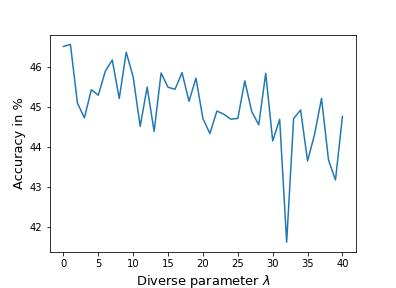
\includegraphics[width=1\linewidth]{fig2fashion}
	  \caption{Dependence of performed accuracy on diversity parameter $\lambda$}
	  \label{fig:graph1fashion}
	\end{subfigure}%
    \hspace{1cm}
	\begin{subfigure}{.46\textwidth}
	  \centering
	  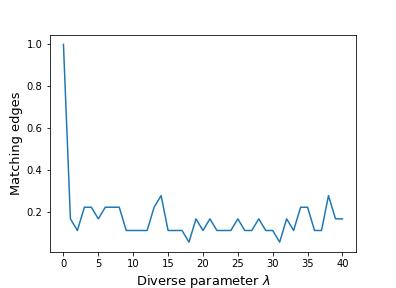
\includegraphics[width=1\linewidth]{fig3fashion}
	  \caption{Dependence of matching edges number on diversity parameter $\lambda$}
	  \label{fig:graph2fashion}
	\end{subfigure}
	\caption{Graphical results of computational experiment on dataset fashionMNIST}
	\label{fig:graphfashion}
\end{figure}

\begin{figure}[H]
	\centering
	\begin{subfigure}{.46\textwidth}
        \centering
	    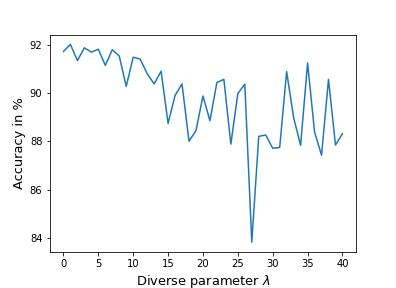
\includegraphics[width=1\linewidth]{fig2CIFAR}
	  \caption{Dependence of performed accuracy on diversity parameter $\lambda$}
	  \label{fig:graph1CIFAR}
	\end{subfigure}%
    \hspace{1cm}
	\begin{subfigure}{.46\textwidth}
	  \centering
	  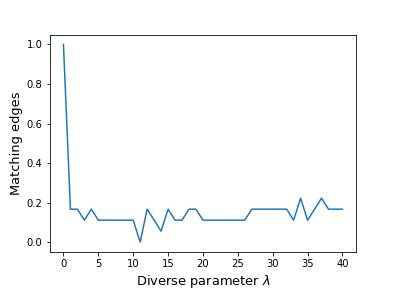
\includegraphics[width=1\linewidth]{fig3CIFAR}
	  \caption{Dependence of matching edges number on diversity parameter $\lambda$}
	  \label{fig:graph2CIFAR}
	\end{subfigure}
	\caption{Graphical results of computational experiment on dataset CIFAR10}
	\label{fig:graphCIFAR}
\end{figure}

Although the instability of the graph presented in \hyperref[fig:graph1fashion]{Fig.2(a)} and \hyperref[fig:graph1CIFAR]{Fig.3(a)} is noticeable, it is evident that the accuracy decreases as the architecture diversity parameter $\lambda$ increases.
However, contrary to our expectations, the amount of intersecting edges depicted in \hyperref[fig:graph2fashion]{Fig.2(b)} and \hyperref[fig:graph2CIFAR]{Fig.3(b)} does not align with our anticipated results.
The reason for this can be attributed to the non-convexity of the optimized function, which causes the algorithm to converge to different minima.
However, we can obtain a higher number of intersecting edges by using a negative $\lambda$.


\subsection{Ensembling effectiveness investigation}

To investigate the effectiveness of ensembling, we employed the following methodology.
We randomly sampled three architectures corresponding to different diverse parameters $\lambda$ chosen randomly and uniformly from a range of 0 to $\Lambda$.
The obtained architectures were then included in an ensemble, and the accuracy of the resulting ensemble was measured.
By changing the diversity limit $\Lambda$, we were able to control the diversity of our deep learning models.
The graphical results of our experiment are depicted in \hyperref[fig:graph4]{Fig.4}.

\begin{figure}[h]
	\centering
	\begin{subfigure}{.46\textwidth}
        \centering
	    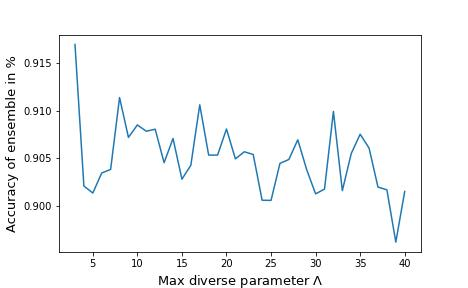
\includegraphics[width=1\linewidth]{fig4fashion}
	  \caption{Experiments on fashionMNIST.}
	  \label{fig:graph4fashion}
	\end{subfigure}%
    \hspace{1cm}
	\begin{subfigure}{.46\textwidth}
	  \centering
	  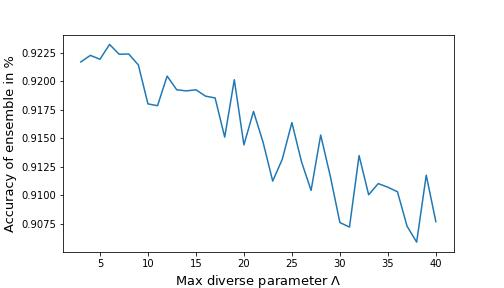
\includegraphics[width=1\linewidth]{fig4CIFAR}
	  \caption{Experiments on CIFAR10.}
	  \label{fig:graph4CIFAR}
	\end{subfigure}
	\caption{\label{fig:graph3} Dependence of effectiveness of deep learning models ensemble on diversity limit $\Lambda$}
	\label{fig:graph4}
\end{figure}

\section{Conclusion}

In this paper, we proposed a novel method for sampling ensembles of deep learning models with diversity control. Our method utilizes a hypernetwork to generate diverse architectures by perturbing a base architecture in terms of Jensen-Shannon divergence. The diversity of the ensemble is controlled by a penalty term added to the loss function, which encourages the ensemble members to be diverse. We conducted experiments on the Fashion-MNIST dataset and demonstrated that our method performs compatible results in terms of accuracy and architectural diversity. Overall, our proposed method shows potential for practical applications in deep learning ensembling.

\bibliography{references}

\end{document}